%%%%%%%%%%%%%%%%%%%%%%%%%%%%%%%%%%%%%%%%%%%%%%%%%%%%%%%%%%%%%
%
% Section: Systems of Linear Equations
%
%%%%%%%%%%%%%%%%%%%%%%%%%%%%%%%%%%%%%%%%%%%%%%%%%%%%%%%%%%%%

\section{Systems of Linear Equations}
\label{SystemsofLinearEquations}

In this chapter we’ve mostly concerned ourselves with linear functions. In this last section we’ll take a look at, and find some uses for, a related but slightly different approach. We’ll begin by
defining some terms.

%%%%%%%%%%%%%%%%%%%%%%%%%%%%%%%%%%%%%%%%%%%%%%%%%%%%%%%%%%%%%
%
% Subsection: Systems of Linear Equations: Graphical Solution
%
%%%%%%%%%%%%%%%%%%%%%%%%%%%%%%%%%%%%%%%%%%%%%%%%%%%%%%%%%%%%

\subsection{Linear Systems and their Solutions}

A linear equation is an equation that either explicitly or implicitly defines a linear function. For example:$$y=3x+5$$
is a linear equation, because if we treat $y$ as the output variable it defines the linear function $f(x)=3x+5$ (which we know is linear because it is written in slope-intercept form.)\\

The equation:$$2x+3y=12$$

is also a linear equation, because it implicitly defines a linear function. We can solve this equation to get:

$$y=-\frac{2}{3}x+4$$

which we can recognize as linear.\footnote{Actually we could just as well have solved for $x$. It’s more common for $y$ to be the output variable, but as we’ve seen before that’s not a requirement.}\\

Usually, we do not need to actually go through the work of solving for one of the variables to see that the equation is linear; usually we can recognize this just by looking at the equation and envisioning what would happen if we solved for one of the variables.\\

A \textbf{system of linear equations, or linear system} \index{System of Linear Equations}, is simply any collection of one or more linear equations. For example:

$$\begin{cases}2x+3y=12\\5x-4y=30\end{cases}$$

is a linear system because it consists of these two linear equations. The bracket that you see on the left side is often used with a linear system to make it clear that these equations are meant to be considered together as a linear system, and not just as two individual equations with no connection to each other. The bracket is not always used in practice, and isn’t required to have a linear system, but it usually is there and in this text we will always do so. \\

A solution to an equation is any pair of values for its variables that satisfy the equation (that is, any pair of values for its variables that make the equation true when substituted in). For example, $x=3$ and $y=2$is a solution for the equation $2x+3y=12$ because when we substitute these values in we get:

$$2(3) + 3(2) = 12 \\ 6 + 6 = 12 \\ 12 = 12$$

which is true. However, this is not a solution to $5x-4y=30$ because if we plug these values into this equation we get:

$$5(3)-4(2)=30\\18-8=30\\7=30$$

which is obviously not true.

A \textbf{simultaneous solution} to a linear system (sometimes just called a \textbf{solution} \index{System of Linear Equations!Solution} to the system) is any pair of values that satisfies all of the equations in the system. For example, $x=3$ and $y=2$ is not a simultaneous solution to the system:

$$\begin{cases}2x+3y=12\\5x-4y=30\end{cases}$$

because we’ve just seen that it does not satisfy both of these equations (it satisfies the first, but not the second.)

One the other hand, $x=6$ and $y=0$ is a simultaneous solution to this system, because both:

$$2(6) + 3(0) = 12\\12 + 0 = 12\\12 = 12$$

and:

$$5(6) - 4(0) = 30\\30 - 0 = 30\\30 = 30$$

are true.\\

We say that we have \textbf{solved} a linear system when we have determined all of its simultaneous solutions.

\subsection{Solving Linear Systems Graphically}

The graphical solution methods we used in Section \ref{LinearFunctionsGraphs} can often be used to solve linear systems.  We will present this method by way of an example, and then give a general description of how to use this method. Read through this example carefully; you’ll probably recognize a lot in the method we will use, though setting things up as a linear system will be new.

\exam{\label{SystemsofLinearEquationsExample1} Menauhant Publishing Company has a contract that costs them a straight $\$80$ per hour for computer support over the phone.  They are considering switching to a new contract that would require them to pay an annual fee of $\$3,000$ regardless of how much service they use, but they would then only be charged $\$50$ per hour.}

\indenttext{If they don’t use much service, obviously their current plan is better. But if they use a lot of service, the new plan would be better. If they were to switch to the new contract, how many hours of service would they have to use to break even on the switch?\\

	We solved this problem in Section \ref{LinearFunctionsGraphs} by setting up a single equation and solving it graphically.  Here, we’ll approach this as a linear system. Cost is a function of hours of service used with either contract, and if we let $y$ be the output (cost) variable and let $x$ be the input (hours of service) variable, we get the following two equations:

	\begin{center}
		Current Contract: $y = 80x$\\
		New Contract: $y = 50x + 3000$
	\end{center}

	To determine the break even between these two options, we need to figure out what number of hours would give the same cost with both of these. So, we need to find out the $x$ (hours) and $y$ (cost) values that would come out the same with both contracts.\\

	In other words, we need to find a simultaneous solution to the linear system:
	$$\begin{cases}	y=80x\\y=50x+3000\end{cases}$$
	Now each of these equations defines a linear function. The graphs of those functions are straight lines consisting of all the points that satisfy their equations. So, the place where the two graphs
	intersect would give the values for the variables that satisfy both equations. Therefore, to find the simultaneous solution to this system, we find the intersection of the two graphs:

	\begin{figure}[H]
		\centering
		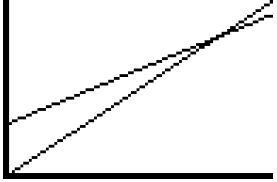
\includegraphics[scale=1.0]{Sections/SystemsofLinearEquationsImages/Figure01.png}
		\caption{graph of $y=80x$ and $y=50x+3000$}
	\end{figure}

	\noindent (For discussion of how to find the appropriate window settings, refer back to Section \ref{SolvingEquationsGraphically}, Solving Equations Graphically)\\

	The solution to this system is $x=100$ and $y=8000$. That is, the break even between these two contracts is $100$ hours of computer support, costing $\$8000$.
}

\bigskip

Solving a linear system graphically is basically the same as solving a linear equation graphically.  The main difference is that, when we are solving a linear system, we start with the two different linear functions – one coming from each equation. We don’t need the step of setting up a linear function based on each side of an equation.\\

The shortcoming of the approach to solving a linear system is that it requires us to have the equations already in a form that explicitly defines a linear function. The system in Example \ref{SystemsofLinearEquationsExample1} had both equations already set up in \quotes{$y=$} form.  When the equations are set up to explicitly define a function, you are ready to go. However, for a linear system whose equations only implicitly define functions, like:

$$\begin{cases}2x+3y=12\\5x-4y=30\end{cases}$$

we would first have to rewrite each equation in explicit function form. The next example will illustrate how this would work.

\exam{\label{SystemsofLinearEquationsExample2} Solve the following linear system graphically: $$\begin{cases}2x+3y=12\\5x-4y=30\end{cases}$$}

\indenttext{We first must rewrite each equation in an explicit function form. So we solve each for $y$.
	$$2x+3y=12\\ \\3y=12-2x\\ \\y=\frac{12-2x}{3}\\ \\y=4-\frac{2}{3}x$$
	and
	$$5x-4y=30\\ \\-4y=30-5x\\ \\y=\frac{30-5x}{-4}\\ \\y=-\frac{15}{2}+\frac{5}{4}x$$
	We now graph these both. Since we don’t have any insights into the meanings of the equations, we’ll simply start with the standard window and adjust if needed to find the intersection.  Fortunately, the standard window works:
	\begin{figure}[H]
		\centering
		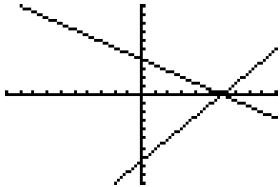
\includegraphics[scale=1.0]{Sections/SystemsofLinearEquationsImages/Figure02.png}
		\caption{Graph to solve system}
	\end{figure}
	\noindent And so we see that the intersection occurs at $(6,0)$ and so conclude that this system’s simultaneous solution is $x=6$ and $y=0$.
}

\bigskip

Most of the time, a given linear system will have one and only one solution.  Each of the equations will define a linear function, those linear functions have graphs that are straight lines, and straight lines can only intersect in one place.  However, sometimes something does go wrong, as we will see in the following example.

\exam{\label{SystemsofLinearEquationsExample3} Solve: $$\begin{cases}x-3y=12\\-2x+6y=-4\end{cases}$$}

\indenttext{Solving the first equation for $y$ we get: 
	$$x-3y=12\\-3y=12-x\\y=\frac{1}{3}x-4$$
	Solving the second equation for $y$ we get:
	$$-2x+6y=4\\6y=4+2x\\y=\frac{2}{3}+\frac{1}{3}x$$
	Looking at these equations in slope-intercept form it is apparent that their graphs are parallel lines.  So there is no point in looking for an intersection; the graphs will never intersect.\\
	\newline
	Therefore, this linear system has no simultaneous solution.
}

\bigskip

So, as this example illustrates, not every linear system will have a solution. Each linear equation has a line as its graph. The lines can intersect once, giving a unique solution to the system. The lines can be parallel, giving no solution. And there is a third possibility: the two lines can turn out to actually be the same. For example, if we were trying to solve the system:

$$\begin{cases} x-3y=12\\-2x+6y=24 \end{cases}$$

We’d see after solving both for $y$ that both of these equations actually turn into the same linear function: $y=\frac{1}{3}x-4$. In this case, since the two equations actually implicitly define the same function, any solution for the one equation also must be a solution for the other. In this case there are infinitely many solutions.\\

In summary, there are three possible results we can run into when solving a linear system:

\begin{center}
	\begin{tabular}{|l|l|}
		\hline
		If the graphs: & Then the linear system has:\\
		\hline
		Have one intersection & One unique solution\\
		\hline
		Are parallel lines & No solutions\\
		\hline
		Are the same line & Infinitely many solutions\\
		\hline
	\end{tabular}
\end{center}

We will now summarize this solution method.

\begin{definition}
	\underline{Solving a Linear System Graphically}\\
	\index{System of Linear Equations!Graphical Solution}	
	\bigskip
	\begin{enumerate}
		\item If the equations are not already in explicit function form, put both equations in this form by solving them for one of the variables. If $y$ is one of the variables, that’s usually the one we solve for. (It does not actually matter which variable you solve for, except that it should be the same one in both equations.)
		\item If both functions have the same slope but different vertical intercepts, the graphs are parallel 	lines. The linear system does not have a solution.
		\item If both functions have the same slope and the same vertical intercept, they are actually both the same function. The system then has infinitely many solutions - any of the infinitely many
		solutions to this equation will actually be a solution to the system.
		\item Otherwise, graph both of the functions on your graphing calculator, and use the methods of graphical solution to find the intersection.
		\item The intersection is the simultaneous solution to the system.
	\end{enumerate}
\end{definition}

Graphical solution always works, but sometimes it is not the most efficient way to solve a linear system. In the rest of this chapter we will present two alternative solution methods.

%%%%%%%%%%%%%%%%%%%%%%%%%%%%%%%%%%%%%%%%%%%%%%%%%%%%%%%%%%%%%
%
% Subsection: Systems of Linear Equations: Substitution
%
%%%%%%%%%%%%%%%%%%%%%%%%%%%%%%%%%%%%%%%%%%%%%%%%%%%%%%%%%%%%

\subsection{Solving Linear Systems by Substitution}

Suppose you are confronted with the following linear system:

$$\begin{cases} 5x+3y=1\\y=2x-7 \end{cases}$$

We could of course solve this graphically. But notice that the second equation is solved for $y$ already. We know from it what $y$ must be in terms of $x$ for any solution to the system. So, we could replace the $y$ in the top equation with the $2x-7$ that we know must be equal to it. If we do this we get:

$$5x+3y=1\\5x+3(2x-7)=1$$

Now the result of doing this is an equation with only one variable, which we can solve with ordinary algebra. We simplify the left side:

$$5x+6x-21=11x-21=11$$

and then finish solving to get:

$$11x=22\\x=2$$

Now this gives us one variable, but we need both to have a complete solution. But since we know $x$ we can substitute that value into either of the original equations and then use that to find $y$. Either one works, but the equation already solved for $y$ would be easiest:

$$y=2x-7\\y=2(2)=7\\y=-3$$

We can generalize and summarize what we’ve done here as a new method for solving linear systems.

\begin{definition}
	\index{System of Linear Equations!Substitution Solution}
	\textbf{\underline{Solving a Linear System by Substitution}}\\
	\bigskip
	\begin{enumerate}
		\item If one of the equations is solved for one variable in terms of the others, start with the next step. Otherwise, solve either one of the equations for one of the variables.
		\item Use the expression that the solved-for variable is equal to as a replacement for the solved for variable in the other equation. The result will be a one variable equation.
		\item Solve the resulting one variable equation. (If the equation has no solution, then the linear system has no solution. If the equation is an identity, then the linear system has infinitely many solutions.)
		\item Substitute the value of the variable you solved for in Step 3 into any of the two variable equations to solve for the original variable.
	\end{enumerate}
\end{definition}

\exam{\label{SystemsofLinearEquationsExample4} I want to fence in a rectangular garden in my back yard. My feng shui adviser tells me the garden will be most harmonious if the length is twice the width. I have $300$ feet of fencing.  What is the largest rectangular and harmonious garden I can enclose with this fencing?}

\indenttext{If we let $W$ represent the width and $L$ the length, we know that the total perimeter is $2L+2W$.  Since that would use the $300$ feet of fencing we must have $2L+2W=300$.  Also, the length is twice the width, so $L=2w$. So we need to solve the linear system:
	$$\begin{cases}2L+2W=300\\L=2W\end{cases}$$	
	The second equation is already solved for $L$, so we use that to substitute into the top equation and solve:
	$$2L+2W=300\\2(2w)+2W=300\\4W+2W=300\\6W=300\\W=50$$
	Now we substitute into the second equation because it is already solved for $L$:
	$$L=2W$$
	$$L=2(50)$$
	$$L=100$$
	So the solution to this system is $W=50$ and $L=100$. In other words, I should fence in a $100 \times 50$ foot garden.
}

\exam{\label{SystemsofLinearEquationsExample5} Use substitution to solve the system: $$\begin{cases} 11T-3P=1\\4P+12T=12	\end{cases} $$}

\indenttext{We need to start by solving one of these equations for one of the variables. We can choose to solve either equation for either variable – the method will work regardless of what we choose.
	However, it makes sense to pick the equation and variable that will be simplest. In the top equation, solving for either variable will involve dividing by either $11$ or $3$, and we can see that this
	will mean fractions will get involved. In the bottom equation solving for $T$ would require us to divide through by $12$, which would make the coefficient of $P$ a fraction. But if we solve for $P$ we will have to divide through by $4$ and since everything in that equation is divisible by $4$ that will avoid fractions. So that seems the cleanest choice.
	\begin{align*}
		4P+12T&=12\\
		4P&=12-12T\\
		P&=3-3T
	\end{align*}
	Now we plug this substitution into the other equation:
	\begin{align*}
		11T-3P&=1\\
		11T-3(3-3T)&=1
	\end{align*}
	And solve the result:
	\begin{align*}
		11T-9+9T&=1\\
		20T-9&=1\\
		20T&=10\\
		T&=\frac{1}{2}
	\end{align*}
	To solve for $P$ we can plug this into either of the original equations. Or, we could use the equation $P=3-3T$ since that is solved for $P$ already. Doing this:
	\begin{align*}
		P&=3-3T\\
		&=3-3(\frac{1}{2})
		&=\frac{3}{2}
	\end{align*}
	So the solution to the system of equations is $P=\frac{3}{2}$ and $T=\frac{1}{2}$.
}

\bigskip

With one last example we will illustrate how things can go wrong. The problem will not be a problem with substitution itself – just like graphing, substitution always works - but there can be problems with the system itself.

\exam{\label{SystemsofLinearEquationsExample6} Solve by substitution $$\begin{cases} x+2z=5\\3x+6z=10 \end{cases}$$}

\indenttext{As before, we can solve for either variable in either equation, but it makes sense to go with the cleanest and simplest choice. In this system, that choice would be to solve for $x$ in the top equation:
	$$x+2z=5\\x=5-2z$$
	Now substitute that into the second equation:
	$$3x+6z=10\\3(5-2z)+6z=10\\15-6z+6z=10\\15=10$$
	This of course is a contradiction. This is not a failure of the substitution method though! When we arrive at a contradiction solving a regular equation, we simply conclude that the equation has no
	solutions. We draw the same conclusion here: the linear system has no solutions. From our previous discussion of solution by graphing, we furthermore know that this means that the graphs of the functions implicitly defined by these two equations must be parallel lines.
}

\bigskip

Two solution methods down, there’s still one more to go:

%%%%%%%%%%%%%%%%%%%%%%%%%%%%%%%%%%%%%%%%%%%%%%%%%%%%%%%%%%%%%
%
% Subsection: Systems of Linear Equations: Substitution
%
%%%%%%%%%%%%%%%%%%%%%%%%%%%%%%%%%%%%%%%%%%%%%%%%%%%%%%%%%%%%

\subsection{Solving Linear Systems by Elimination}

Suppose you are presented with the linear system:

$$\begin{cases} 5x+2y=1\\3x-2y=7 \end{cases}$$

This system can of course be solved by graphing or by substitution, though either method will require some effort. Here, a third possibility presents itself. Notice that the $y$ terms in the two equations are just the opposite sign of each other - almost begging us to find a way to cancel each out against the other.\\

Now, the second equation says that $3x-2y$ is equal to $7$. This is a big deal. This means that even though $3x+2y$ and $7$ look quite different, they actually have the same value. So if I were to
add $3x+2y$ to one side of some other equation, and add $7$ to the other side, this would be OK because I’d be adding equal things to both sides.\\

That is precisely what I want to do. We will take the top equation, and add $3x+2y$ to its left side, and $7$ to its right:

\begin{center}
	\begin{tabular}{c@{\,}c@{\,}c@{\,}c@{\,}c@{\,}c}
		& 5x &+ & 2y & = & 1 \\
		+ & (3x &- & 2y) & & +7 \\
		\hline
		& 8x & + & 0y & = & 8 \\
	\end{tabular}
\end{center}

So by doing this we’ve created a new equation where one of the variables ($y$) has been eliminated!  The result is easily solved for the remaining variable:

$$8x=8$$

$$x=1$$

So we have our $x$. Now to get the other variable, we can substitute this value for $x$ into either of the original equations:

\begin{equation*}
	5x+2y=1\\
	5(1)+2y=1\\
	5+2y=1\\
	2y=-4\\
	y=-2
\end{equation*}

So we’ve solved this system: $x=1$ and $y=-2$.\\

Now this was a pretty special case. This approach worked because the coefficients of $y$ in the two equations just happened to be $\pm$ of each other. That usually won’t happen. But we can force it to happen if we want to. Suppose we were up against the system:

$$\begin{cases} 2p+7q=9\\p+3q=5 \end{cases}$$

If we were to multiply both sides of the bottom equation through by $-2$ we’d make the $p$ term of that equation $-2p$, perfectly set up to cancel with the top equation’s $2p$:

$$\begin{cases} 2p+7q=9\\-2(p+3q)=-2(5) \end{cases}$$

which makes the system become:

$$\begin{cases} 2p+7q=9\\-2p-6q=-10 \end{cases}$$

and we could proceed as before, adding the left side of the bottom equation to the left side of the top, and the right side of the bottom to the right side of the top to get:

\begin{center}
	\begin{tabular}{c@{\,}c@{\,}c@{\,}c@{\,}c@{\,}c}
		& 2p & + & 7q & = & 9 \\
		+ & (-2p & - & 6y) & & (-10) \\
		\hline
		&  &  & q & = & -1 \\
	\end{tabular}
\end{center}

So the value of $q$ actually falls out here beautifully. Plugging it back into either of the original equations we can solve for $p$, and when you do that you will end up with the solution to this system:  $p = 8$ and $q = -1$.\\

Now in this system multiplying the bottom equation by $-2$ and eliminating $p$ was the simplest solution. But we could have done it other ways too. For example, if we had multiplied the top equation by $3$ and the bottom one by $-7$ we would have gotten:

\begin{equation*}
	\begin{cases}
		3(2p+7q)=3(9)\\
		-7(p+3q)=-7(5)
	\end{cases}
	\text{    which becomes    }
	\begin{cases}
		6p+21q=27\\
		-7p-21q=-35
	\end{cases}
\end{equation*}

which is set up to eliminate $q$ which will work out just as well. The point here is that if we need to, we can multiply through one or both of the equations in a system to set up one of the variables for elimination. Let’s generalize this method before looking at another example:

\begin{definition}
	\index{System of Linear Equations!Elimination Solution}
	\textbf{\underline{Solving a Linear System by Elimination}}\\
	\bigskip
	\begin{enumerate}
		\item If necessary, rearrange the equations so that the corresponding variables line up.
		\item If one of the variables has coefficients that are $\pm$ of each other in the two equations, continue with the next step. If not, multiply both sides of one equation or of both equations
		by something so that one of the variables will have coefficients that are $\pm$ each other.
		\item Add the corresponding sides of the equations. The result should be a one variable equation. You’ve \quotes{eliminated} one of the variables. (If the result is a contradiction, the system has no solutions. If the result is an identity, the system has infinitely many solutions.)
		\item Solve the resulting one variable equation.
		\item Substitute the value of the solved for variable into one of the original equations, and solve for the remaining variable.
	\end{enumerate}
\end{definition}

\exam{\label{SystemsofLinearEquationsExample7} Solve by elimination:$$\begin{cases} 5p-7q=14\\12p+8q=-16 \end{cases}$$}

\indenttext{In this system the variables are already lined up $p$ above $p$ and $q$ above $q$ so we are ready to go.  We can choose to eliminate either variable; in this case neither one is really a better choice than the other. If we want to eliminate $p$ we could multiply the top equation through by $12$ and the bottom through by $-5$, or the top by $-12$ and the bottom by $5$, to make the $p$ terms $\pm 60p$. Or we could eliminate $q$ by multiplying the top by $8$ and the bottom by $7$ to make the $q$ terms $\pm56q$.\\

For no particular reason, we’ll take the path that eliminates $q$:
\begin{equation*}
	\begin{cases}
		8(5p-7q)=8(14)\\
		7(12p+8q)=7(-16)
	\end{cases}
	\text{    which becomes    }
	\begin{cases}
		40p-56q=112\\
		84p+56q=-112
	\end{cases}
\end{equation*}

and now we add the corresponding sides of the system to get:

\begin{center}
	\begin{tabular}{c@{\,}c@{\,}c@{\,}c@{\,}c@{\,}c}
		& 40p & - & 56q & = & 112 \\
		+ & 84p & + & 56q) & & -112 \\
		\hline
		& 124p &  &  & = & 0 \\
	\end{tabular}
\end{center}

which we now solve to conclude that:
$$p=0$$
Substituting this into either equation (for no particular reason we’ll choose the top one):

\begin{align*}
	5p-7q&=14\\
	5(0)-7q&=14\\
	-7q&=14\\
	q&=-2
\end{align*}

So the system’s solution is $p = 0$ and $q = -2$.
}

%%%%%%%%%%%%%%%%%%%%%%%%%%%%%%%%%%%%%%%%%%%%%%%%%%%%%%%%%%%%%
%
% Subsection: Systems of Linear Equations: Strategies for Solving Linear Systems
%
%%%%%%%%%%%%%%%%%%%%%%%%%%%%%%%%%%%%%%%%%%%%%%%%%%%%%%%%%%%%

\subsection{Strategies for Solving Linear Systems}

So we now have three methods to solve linear systems. All three methods always work - no matter which method you choose to use, if the system has a solution you will find it, and if there is no
solution or are infinitely many solutions each system has a way of telling you that as well. So, in the face of a given linear system, how do you choose which method to use?\\

Even though all three methods will work on any system, it is often the case that one of them will be a lot less work than the others. For example, the system: is set up beautifully for a graphical solution (just letting $w$ become the Y and $z$ the X in your graphing calculator.\\

This system is also set up nicely for substitution, since both equations are already solved for $w$, making it easy to replace the $w$ in either equation to get the equation

$$3z-1=-5z+2$$

Actually elimination would also work pretty nicely with this system (just multiply both sides of either equation through by $-1$), though given how nicely this is set up for the other methods elimination
probably would not be the preferred way to go.\\

For a different example, consider this system:

$$\begin{cases}5p-4q=3\\p=q+1 \end{cases}$$

Now with this system, graphing would work, but it would require solving the top equation for $p$ to start. That’s not too difficult, but it would take a bit of algebra effort, and would introduce fractions.  Not too bad, but not nearly as simple as noticing that the second equation is already solved for $p$ in terms of $q$. Given that, it would be simple to use this to substitute into the top equation to get $5(q+1)-4q=3$ which is not a hard equation to solve. \\

Elimination on the other hand would take more doing. We would first have to rearrange the bottom equation so that the variables would line up, getting:

$$\begin{cases}5p-4q=3\\p-q=1 \end{cases}$$

and then proceeding. Now this actually is a pretty straightforward elimination problem, but the effort of rearranging and then doing the elimination seems to me to be much greater than the effort required to do substitution right from the start.\\

Now, which method would be the best bet with this system?

$$\begin{cases}3x-11y=28\\2x-9y=22\end{cases}$$

For this graphing would require solving both equations for one of the variables, requiring a fair amount of algebra and a fair amount of fractions. Not the end of the world, but maybe not too desirable if we can avoid it.\\

Substitution would probably not go well. Solving either equation for one of the variables would involve some messiness. The best bet would be to solve the second equation for $x$, which would give $x=\frac{9}{2}y+11$ which would then be substituted into the top equation to get $3(\frac{9}{2}y+11)-11=28$. Again not the end of the world, but not too much fun, either.\\

On the other hand, this system is beautifully set up for elimination. Multiplying the top through by $2$ and the bottom by $-3$ would set this up for a nice, clean, elimination of the $x$.  Now in each of these examples, it really doesn’t matter which method you use. Again, any method will work on any system, so you never have to worry that you’ll make the \quotes{wrong choice} and then be unable to solve the system because of your choice. But when confronted with a new system to solve it is worth spending a moment or two to think through how each method would play out.  Investing a moment or two to strategize your solution method can save you unnecessary effort. \\

In the exercises for this section, you will find many problems where you are asked to solve a linear system by a specific method. It is important that you know how to use all three methods so that you have all three at your disposal, and also because each of the three methods can be generalized to other uses in mathematics. (For example, substitution can be used even if the equations in a system are non-linear, but elimination does not work so well in that case; while elimination adapts readily to linear systems with more than two variables while substitution does not do so nearly as well and graphing is hopeless!) For this reason, if a specific method is called for, you must use that method.\\

In other problems, though, you have your choice. In those cases, choose wisely! Making a good choice of method can save you an awful lot of needless effort.

%%%%%%%%%%%%%%%%%%%%%%%%%%%%%%%%%%%%%%%%%%%%%%%%%%%%%%%%%%%%%
%
% Subsection: System of Linear Equations: Exercises
%
%%%%%%%%%%%%%%%%%%%%%%%%%%%%%%%%%%%%%%%%%%%%%%%%%%%%%%%%%%%%%

\clearpage
\subsection{Exercises}

\subsubsection*{Linear Systems and their Solutions}

\bigskip
\ex{Determine whether or not each of the given input-output pairs is a solution to the linear system.
	$$\begin{cases}x+3y=5\\x-2y=0\end{cases}$$
	\begin{enumerate}[label=(\alph*)]
		\item $x=5$, $y=0$
		\item $x=2$, $y=1$
		\item $x=1$, $y=1$
		\item $x=3$, $y=-1$
	\end{enumerate}	
}
\sol{a,c, and d are not; b is}

\bigskip
\ex{Determine whether or not each of the given input-output pairs is a solution to the linear system.
	$$\begin{cases}2x+3y=11\\x-5y=25\end{cases}$$
	\begin{enumerate}[label=(\alph*)]
		\item $x=10$, $y=3$
		\item $x=-10$, $y=7$
		\item $x=-10$, $y=-7$
		\item $x=10$, $y=-3$
	\end{enumerate}	
}

\bigskip
\ex{Ticket prices for a play cost $\$15$ for kids under 12 and $\$25$ for everyone else. Two hundred tickets were sold for a total of $\$4200$. Let $k$ be the number of kids’ tickets and let $a$ be the number of regular tickets sold.  Based on this information, the number of tickets sold must satisfy the equations $k+a=200$ and $15k+25a=4200$.  Which of the following could be the number of each type ticket sold?
	\begin{enumerate}[label=(\alph*)]
		\item $50$ kids tickets and $150$ regular
		\item $100$ of each type of ticket
		\item $80$ kids tickets and $120$ regular 
		\item $80$ regular and $120$ kids tickets.
	\end{enumerate}
}
\sol{c is possible; a, b, and d are not}

\bigskip
\ex{Ticket prices for a play cost $\$10$ for kids under $12$ and $\$25$ for everyone else. Two hundred tickets were sold for a total of $\$3500$. Let $k$ be the number of kids’ tickets and let $a$ be the number of regular tickets sold.  Based on this information, the number of tickets sold must satisfy the equations $k+a=200$ and $10k+25a=3500$.  Which of the following could be the number of each type ticket sold?
	\begin{enumerate}[label=(\alph*)]
		\item $50$ kids tickets at $150$ regular 
		\item $100$ of each type of ticket
		\item $80$ kids tickets and $120$ regular
		\item $80$ regular and $120$ kids tickets.
	\end{enumerate}
}

\subsubsection*{Solving Linear Systems Graphically}

Solve each of the following linear systems graphically. When necessary, express your final answers either with fractions in lowest terms or decimals rounded to two places.

\bigskip
\ex{$\begin{cases}y=3x+2\\y=5x-2\end{cases}$}
\sol{$x=2$ and $y=8$}

\bigskip
\ex{$\begin{cases}y=-2x+2\\y=7x-7\end{cases}$}

\bigskip
\ex{$\begin{cases}x+y=5\\8x-2y=0\end{cases}$}
\sol{$x=1$ and $y=4$}

\bigskip
\ex{$\begin{cases}4y-x=8\\2y+4x=13\end{cases}$}

\bigskip
\ex{$\begin{cases}3M-2N=16\\8M+2N=6\end{cases}$}
\sol{$M=2$ and $N=-5$}

\bigskip
\ex{$\begin{cases}3K+5E=9\\2K-11E=6\end{cases}$}

\bigskip
\ex{$\begin{cases}4x+2y=0\\6x=5-3y\end{cases}$}
\sol{No solutions}

\bigskip
\ex{$\begin{cases}F-3G=5\\2F=6G+10\end{cases}$}

\subsubsection*{Solving Linear Systems by Substitution}

Solve each of the following linear systems by substitution. When necessary, express your final answers either with fractions in lowest terms or decimals rounded to two places.

\bigskip
\ex{$\begin{cases}3x-7y=2\\y=2x-5 \end{cases}$}
\sol{$x=3$ and $y=1$}

\bigskip
\ex{$\begin{cases}2y-5x=21\\y=x-2 \end{cases}$}

\bigskip
\ex{$\begin{cases}R=4S-3\\2R-6S=-42 \end{cases}$}
\sol{$R=-75$ and $S=-18$}

\bigskip
\ex{$\begin{cases}z=5y+1\\ 24=2z-4y\end{cases}$}

\bigskip
\ex{$\begin{cases}3t+2p=9\\2t+2p=16 \end{cases}$}
\sol{$t=-7$ and $p=15$}

\bigskip
\ex{$\begin{cases}6h+2q=10\\7h-3q=1 \end{cases}$}

\bigskip
\ex{$\begin{cases}15t-6w=36\\5t=12+2w \end{cases}$}
\sol{identity; infinitely many solutions}

\bigskip
\ex{$\begin{cases}3x-4z=13\\12z-9x=9 \end{cases}$}

\subsubsection*{Solving Linear Systems by Elimination}

Solve each of the following linear systems by elimination. When necessary, express your final answers either with fractions in lowest terms or decimals rounded to two places.

\bigskip
\ex{$\begin{cases}3x-5y=11\\4x+5y=3 \end{cases}$}
\sol{$x=2$ and $y=-1$}

\bigskip
\ex{$\begin{cases}2x+9y=5\\-2x-7y=3 \end{cases}$}

\bigskip
\ex{$\begin{cases}2x+5y=11\\x-3y=0 \end{cases}$}
\sol{$x=3$ and $y=1$}

\bigskip
\ex{$\begin{cases}3x-2y=5\\x+5y=7 \end{cases}$}

\bigskip
\ex{$\begin{cases}5y-4x=18\\10y-8x=36 \end{cases}$}
\sol{identity; infinitely many solutions}

\bigskip
\ex{$\begin{cases}x+3y=7\\2x+6y=14 \end{cases}$}

\bigskip
\ex{$\begin{cases}3A+5B=2\\4A+8B=0 \end{cases}$}
\sol{$A=4$ and $B=-2$}

\bigskip
\ex{$\begin{cases}9t-4p=7\\-5t+6p=1 \end{cases}$}

\bigskip
\ex{$\begin{cases}12z+11t=19\\30z+8t=25 \end{cases}$}
\sol{$t=\frac{45}{39}$ and $z\frac{41}{78}$}

\bigskip
\ex{$\begin{cases}15p-36q=0\\12p-17q=25 \end{cases}$}

\subsubsection*{Strategies for Solving Linear Systems}

Decide which solution method you feel would be the best approach to solving each of the following linear systems. You do not need to actually solve them.

\bigskip
\ex{$\begin{cases}3x+2y=11\\2x-7y=9 \end{cases}$}
\sol{elimination is probably the best}

\bigskip
\ex{$\begin{cases}3x-7y=15\\x=2+y \end{cases}$}

\bigskip
\ex{$\begin{cases}y=3x-5\\y=x+2 \end{cases}$}
\sol{any of the three methods would be fine; graphing and substitution are probably the best}

\bigskip
\ex{$\begin{cases}100x-30y=500\\40x+45y=800 \end{cases}$}

\bigskip
\ex{$\begin{cases}5x+8p=15\\x-2p=8 \end{cases}$}
\sol{elimination would probably be the best choice, but substitution would also work well}

\bigskip
\ex{$\begin{cases}p=2m-1\\p=11-6m \end{cases}$}

\bigskip
\ex{$\begin{cases}6t-8p=5\\p=3t+1 \end{cases}$}
\sol{substitution since the second equation is already solved for one of the variables}

\bigskip
\ex{$\begin{cases}t=5k+1\\16t-11k=8 \end{cases}$}

\bigskip
\ex{$\begin{cases}J=3K+9\\3J+11K=-6 \end{cases}$}
\sol{substitution since the first equation is already solved for one of the variables}

\bigskip
\ex{$\begin{cases}r-3(s+2)=11\\5r-3s=8-2r \end{cases}$}

\bigskip
\ex{$\begin{cases}N-3M=19\\N+4M=17 \end{cases}$}
\sol{elimination would be a very good choice, but either substitution or graphing would also work well.}

\bigskip
\ex{$\begin{cases}3f+9p=0\\5f-2p=7 \end{cases}$}

\bigskip
\ex{$\begin{cases}x=4y-1\\x=5-2y \end{cases}$}
\sol{any of the three methods would be fine, but graphing or substitution would probably be best}

\subsubsection*{Grab Bag}

Solve each of the following problems. You may use your choice of methods. When necessary, express your final answers either with fractions in lowest terms or decimals rounded to two places.

\bigskip
\ex{Solve $\begin{cases}3t-11p=22\\6t-5p=10 \end{cases}$}

\bigskip
\ex{Solve $\begin{cases}5x+y=16\\x=11y-8 \end{cases}$}
\sol{$x=3$ and $y=1$}

\bigskip
\ex{Solve $\begin{cases}2x+5y=20\\2x=y+8 \end{cases}$}

\bigskip
\ex{Solve $\begin{cases}x=3y+1\\x=4y-2 \end{cases}$}
\sol{$x=10$ and $y=3$}

\bigskip
\ex{Solve $\begin{cases}h=9-2t\\h=t+1 \end{cases}$}

\bigskip
\ex{Solve $\begin{cases}6x+2y=22\\5x+3y=45 \end{cases}$}
\sol{$x=-3$ and $y=20$}

\bigskip
\ex{An office manager needs to buy software licenses. The vendor only sells licenses in packs. A \quotes{Professional Pack} includes $5$ spreadsheet and $10$ word processing licenses. An \quotes{Analyst Pack} includes $12$ spreadsheet and $8$ word processing licenses.
	\begin{enumerate}[label=(\alph*)]
		\item Let $P$ be the number of Professional Packs he buys, and let $A$ be the number of Analyst Packs he buys. Write an algebraic expression which gives the number of spreadsheet licenses he would receive.
		\item Using the same variables as in $(a)$ write an algebraic expression which gives the number of word processing licenses he would receive.
		\item Suppose he needs $200$ spreadsheet licenses and $240$ word processing licenses.  Use your answers to $(a)$ and $(b)$ together with this information to write two equations.
		\item Solve the linear system you got from $(c)$. How many of each type of license pack should the office manager order?
	\end{enumerate}
}

\bigskip
\ex{Tim has just gone on the SuperCarboStarver Diet. He must plan his meals to precisely contain the exact amounts of fat and protein that the diet calls for. He has two types of food to eat for lunch. Each serving of B-B-Q pork rinds contains $5$ grams of fat and $2$ gram of protein. Each Teriyaki Turkey Jurkey Stick contains $2$ grams of fat at $6$ grams of protein.
	\begin{enumerate}[label=(\alph*)]
		\item Let $P$ be the number of servings of pork rinds he will eat, and let $J$ be the number of turkey jurkey sticks. Write an algebraic expression which gives the number of grams of fat he will get from his meal.
		\item Using the same variables as in $(a)$ write an algebraic expression for the number of grams of protein he will get.
		\item Suppose that according to his diet he should eat $20$ grams of fat and $34$ grams of protein for dinner. Use your answers to $(a)$ and $(b)$ together with this information two write as system of two equations.
		\item Solve the linear system you got from $(c)$. What should Tim have for dinner?
	\end{enumerate}
}
\sol{a.  $5P+2J$\\b. $2P+6J$\\c.  $\begin{cases}5P+2J=20\\2P+6J=34 \end{cases}$\\d.  a green salad and a diet sprite.  But according to this linear system he should have 5 turkey jurkey sticks and two servings of pork rinks.}

\bigskip
\ex{Katrina set out to solve the linear system:  $$\begin{cases}2x-y=7\\3x+2y=28 \end{cases}$$ using substitution.  She solved the first equation for $y$ to get:  $$y=2x-7$$ and then substituted to get:  \begin{align*} 2x-y&=7 \\ 2x-(2x-7)&=7 \\ 7=7 \end{align*} and so, she concluded, since this is an identity, that the linear system has infinitely many solutions.  However, the correct answer is that this system has only one solution, $x=6$ and $y=5$.  Where did she go wrong?}

\clearpage
